% !TeX spellcheck = en_GB
%%%%%%%%%%%%%%%%%%%%%%%%%%%%%%%%%%%%%%%%%%
%                                        %
%    Engineer thesis LaTeX template      % 
%                                        %
%%%%%%%%%%%%%%%%%%%%%%%%%%%%%%%%%%%%%%%%%%



\documentclass[a4paper,twoside,12pt]{book}
\usepackage[utf8]{inputenc}                                      
\usepackage[T1]{fontenc}  
\usepackage{amsmath,amsfonts,amssymb,amsthm}
\usepackage[polish,british]{babel} 
\usepackage{indentfirst}
\usepackage{lmodern}
\usepackage{graphicx} 
\usepackage{hyperref}
\usepackage{booktabs}
\usepackage{tikz}
\usepackage{pgfplots}
\usepackage{mathtools}
\usepackage{geometry}
\usepackage[page]{appendix} 

\usepackage{setspace}
\onehalfspacing


\frenchspacing

\usepackage{listings}
\lstset{
	language={},
	basicstyle=\ttfamily,
	keywordstyle=\lst@ifdisplaystyle\color{blue}\fi,
	commentstyle=\color{gray}
}

%%%%%%%%%

 

%%%%%%%%%%%% FANCY HEADERS %%%%%%%%%%%%%%%

\usepackage{fancyhdr}
\pagestyle{fancy}
\fancyhf{}
\fancyhead[LO]{\nouppercase{\it\rightmark}}
\fancyhead[RE]{\nouppercase{\it\leftmark}}
\fancyhead[LE,RO]{\it\thepage}


\fancypagestyle{onlyPageNumbers}{%
   \fancyhf{} 
   \fancyhead[LE,RO]{\it\thepage}
}

\fancypagestyle{PageNumbersChapterTitles}{%
   \fancyhf{} 
   \fancyhead[LO]{\nouppercase{\it\rightmark}}
   \fancyhead[RE]{\nouppercase{\it\leftmark}}
   \fancyhead[LE,RO]{\it\thepage}
}


%%%%%%%%%%%%%%%%%%%%%%%%%%%
% listings 
\usepackage{listings}
\lstset{%
language=C++,%
commentstyle=\textit,%
identifierstyle=\textsf,%
keywordstyle=\sffamily\bfseries, %\texttt, %
%captionpos=b,%
tabsize=3,%
frame=lines,%
numbers=left,%
numberstyle=\tiny,%
numbersep=5pt,%
breaklines=true,%
morekeywords={descriptor_gaussian,descriptor,partition,fcm_possibilistic,dataset,my_exception,exception,std,vector},%
escapeinside={@*}{*@},%
%texcl=true, % wylacza tryb verbatim w komentarzach jednolinijkowych
}
%%%%%%%%%%%%%%%%%%%%%%%%%%%%%%%%%%%%

%%%% TODO LIST GENERATOR %%%%%%%%%

\usepackage{color}
\definecolor{brickred}      {cmyk}{0   , 0.89, 0.94, 0.28}

\makeatletter \newcommand \kslistofremarks{\section*{Remarks} \@starttoc{rks}}
  \newcommand\l@uwagas[2]
    {\par\noindent \textbf{#2:} %\parbox{10cm}
{#1}\par} \makeatother


\newcommand{\remark}[1]{%
{%\marginpar{\textdbend}
{\color{brickred}{[#1]}}}%
\addcontentsline{rks}{uwagas}{\protect{#1}}%
}

%%%%%%%%%%%%%% END OF TODO LIST GENERATOR %%%%%%%%%%% 

% some issues...

\newcounter{PagesWithoutNumbers}

\newcommand{\hcancel}[1]{%
    \tikz[baseline=(tocancel.base)]{
        \node[inner sep=0pt,outer sep=0pt] (tocancel) {#1};
        \draw[red] (tocancel.south west) -- (tocancel.north east);
    }%
}%

\newcommand{\MonthName}{%
  \ifcase\the\month
  \or January% 1
  \or February% 2
  \or March% 3
  \or April% 4
  \or May% 5
  \or June% 6
  \or July% 7
  \or August% 8
  \or September% 9
  \or October% 10
  \or November% 11
  \or December% 12
  \fi}


%%%%%%%%%%%%%%%%%%%%%%%%%%%%%%%%%%%%%%%%%%%%%%
% Helvetica font macros for the title page:
\newcommand{\headerfont}{\fontfamily{phv}\fontsize{18}{18}\bfseries\scshape\selectfont}
\newcommand{\titlefont}{\fontfamily{phv}\fontsize{18}{18}\selectfont}
\newcommand{\otherfont}{\fontfamily{phv}\fontsize{14}{14}\selectfont}

%%%%%%%%%%%%%%%%%%%%%%%%%%%%%%%%%%%%%%%%%%%%%%
%%%%%%%%%%%%%%%%%%%%%%%%%%%%%%%%%%%%%%%%%%%%%%
%%%%%%%%%%%%%%%%%%%%%%%%%%%%%%%%%%%%%%%%%%%%%%
%%%%%%%%%%%%%%%%%%%%%%%%%%%%%%%%%%%%%%%%%%%%%%
%%%%%%%%%%%%%%%%%%%%%%%%%%%%%%%%%%%%%%%%%%%%%%
%%%%%%%%%%%%%%%%%%%%%%%%%%%%%%%%%%%%%%%%%%%%%%
%%%%%%%%%%%%%%%%%%%%%%%%%%%%%%%%%%%%%%%%%%%%%%
\newcommand\tabularhead[1]{
\begin{table}[h]
  \caption{Action <<#1>>}
  \begin{tabular}{|p{0.4\linewidth}|p{0.55\linewidth}|}
    \hline
    \textbf{Action} & \textbf{#1} \\
    \hline}

  \newcommand\addrow[2]{#1 &#2\\ \hline}

  \newcommand\addmulrow[2]{ \begin{minipage}[t][][t]{2.5cm}#1\end{minipage}% 
     &\begin{minipage}[t][][t]{8cm}
      \begin{enumerate} #2   \end{enumerate}
      \end{minipage}\\ }

  \newenvironment{usecase}{\tabularhead}
{\hline\end{tabular}\end{table}}

\newcommand{\Author}{Adam Gajewski}
\newcommand{\Supervisor}{Krzysztof Dobosz, DSc PhD}
%\newcommand{\Consultant}{Name Surname, PhD}
\newcommand{\Title}{Accessible Sudoku}
\newcommand{\Polsl}{Silesian University of Technology}
\newcommand{\Faculty}{Faculty of Automatic Control, Electronics and Computer Science}


\begin{document} 
	
%%%%%%%%%%%%%%%%%%  Title page %%%%%%%%%%%%%%%%%%% 
\pagestyle{empty}
{
	\newgeometry{top=2.5cm,%
	             bottom=2.5cm,%
	             left=3cm,
	             right=2.5cm}
	\sffamily
	\rule{0cm}{0cm}
	
	\begin{center}
	
\includegraphics[width=29mm]{polsl}
	\end{center} 
	\vspace{1cm}
	\begin{center}
	\headerfont \Polsl
	\end{center}
	\begin{center}
	\headerfont \Faculty
	\end{center}
	\vfill
	\begin{center}
	\titlefont Engineer  thesis
	\end{center}
	\vfill
	
	\begin{center}
	\otherfont \Title\par
	\end{center}
	
	\vfill
	
	\vfill
	 
	\noindent\vbox
	{
		\hbox{\otherfont author: \Author}
		\vspace{12pt}
		\hbox{\otherfont supervisor: \Supervisor}
		\vspace{12pt}
		%\hbox{\otherfont consultant: \Consultant}
	}
	\vfill 
 
   \begin{center}
   \otherfont Gliwice,  \MonthName\ \the\year
   \end{center}	
	\restoregeometry
}
  

\cleardoublepage
 

\rmfamily
\normalfont


%%%%%%%%%%%% statements required by law and Dean's office %%%%%%%%%%
\cleardoublepage

\begin{flushright}
załącznik nr 2 do zarz. nr 97/08/09 
\end{flushright}

\vfill  

\begin{center}
\Large\bfseries Oświadczenie
\end{center}

\vfill

Wyrażam  zgodę / Nie wyrażam zgody*  na  udostępnienie  mojej  pracy  dyplomowej / rozprawy doktorskiej*.

\vfill

Gliwice, dnia {\selectlanguage{polish}\today}

\vfill

\rule{0.5\textwidth}{0cm}\dotfill 

\rule{0.5\textwidth}{0cm}
\begin{minipage}{0.45\textwidth}
{\begin{center}(podpis)\end{center}}
\end{minipage} 

\vfill

\rule{0.5\textwidth}{0cm}\dotfill 

\rule{0.5\textwidth}{0cm}
\begin{minipage}{0.45\textwidth}
{\begin{center}\rule{0mm}{5mm}(poświadczenie wiarygodności podpisu przez Dziekanat)\end{center}}
\end{minipage}


\vfill

* podkreślić właściwe

 


%%%%%%%%%%%%%%%%%%%%%  
\cleardoublepage

\rule{1cm}{0cm}

\vfill  

\begin{center}
\Large\bfseries Oświadczenie promotora
\end{center}

\vfill

Oświadczam, że praca „\Title” spełnia wymagania formalne pracy dyplomowej inżynierskiej.

\vfill



\vfill

Gliwice, dnia {\selectlanguage{polish}\today}

\rule{0.5\textwidth}{0cm}\dotfill 

\rule{0.5\textwidth}{0cm}
\begin{minipage}{0.45\textwidth}
{\begin{center}(podpis promotora)\end{center}}
\end{minipage} 

\vfill
 
 

\cleardoublepage


%%%%%%%%%%%%%%%%%% Table of contents %%%%%%%%%%%%%%%%%%%%%%
\pagenumbering{Roman}
\pagestyle{onlyPageNumbers}
\tableofcontents

%%%%%%%%%%%%%%%%%%%%%%%%%%%%%%%%%%%%%%%%%%%%%%%%%%%%%
\setcounter{PagesWithoutNumbers}{\value{page}}
\mainmatter
\pagestyle{PageNumbersChapterTitles}

%%%%%%%%%%%%%% body of the thesis %%%%%%%%%%%%%%%%%


\chapter{Introduction}

\begin{itemize}
\item introduction into the problem domain
\item settling of the problem in the domain
\item objective of the thesis 
\item scope of the thesis
\item short description of chapters
%\item clear description of contribution of the thesis's author – in case of more authors table with enumeration of contribution of authors
\end{itemize}


\clearpage

\section{Introduction into the problem domain\\{\large Short description of accessibility}}
\par
Accessibility is a feature that lets blind people to use smartphones. Even if an app was not designed for blind people, they mostly still can use it thanks to screen readers like Talkback (an accessibility service for Android) reading out loud the content of app to the user. It is a small help compere to many problems connected to being blind, but we can increase this help, by creating applications that are more accessible friendly.
\par
Due to the fact that in order to know what is the content of something that is currently displayed on the screen, a specific part of the screen must be tapped, the application should not use the same event as the chose action. In Talkback this event is overwritten by double tap, so after first tap a button (for example) Talkback tells the user what was just tapped. After a double tap the application calls the same action as if this element was tapped once with Talkback turned off. Using Talkback changes this and many other behaviors of applications, which can make many applications unable to work properly. To change this back to how the application worked originally without Talkback, the application have to be designed either disable some of Talkback features for parts of itself, or overwrite its reactions to touch events.
\par
The easiest accessible thing to implement is some text to read. To any other elements should be provided appropriate labels. Thanks to that most of visual features can be forgotten and the user can proceed to use the app. One of problems of this solution is time necessary for the audio to be played. Because of that application requiring faster response are a lot harder to be accessible, so there are not many accessible games on smartphones.

\section{Settling of the problem in the domain\\{\large Short description of accessible games in general}}
\par
Making an accessible game we can take one of two approaches: Either we make the UI simple and decrease number of elements on screen to minimum, or we take the risk of making something more complicated. In the first case we just have to think of an idea that does not require from the user to chose from many options or to react very fast. It leaves us with really lot of options: Quizzes, text RPG's, crosswords, and so on. Simple design does not make a game boring, everything depends on the execution. In the second case we must put trust in the user and make a bit more complicated UI with more elements. When the user will get used to the game this difference in difficulty should decrease, but the time for learning how to play will be usually longer, than in the first case.

\section{Objective of the thesis}%\\{\large Short description of what the game should be}}

\par The main objective is to create a working accessible Sudoku game that can be solved both by a blind person and someone fully sighted.

\iffalse
\titleformat{\chapter}[display]
  {\normalfont\sffamily\huge\bfseries}
  {\chaptertitlename\ \thechapter}{5pt}
  {\begin{flushleft}
  \normalfont\normalsize\textit{Here is the place where the description of each chapter goes. \vspace{0.25cm}}
  \end{flushleft}
  \Huge}
\fi
\chapter{[Problem analysis]}



\begin{itemize}
\item  problem analysis
\item state of the art, problem statement
\item  literature research (all sources in the thesis have to be referenced \cite{bib:article,bib:book,bib:conference,bib:internet})
\item description of existing solutions (also scientific ones, if the problem is scientifically researched), algorithms,  location of the thesis in the scientific domain
\end{itemize}

\clearpage

\section {Problem Analysis\\{\large Description of some accessible solutions}}

\par
The smartphone accessible games have been available for a few years, and the conventional ones were more common for even longer. Puzzles like Rubik cube with braille alphabet on it can be found easily, and there exists a similar solution for the Sudoku puzzle, with numbers represented by small blocks with braille number on it, that can be putted into the puzzle. That solution can not be used in an electronic device not having any form of system showing braille alphabet. There exists a solution on the descktop computer using keyboard and audio reading content of the sudoku, but agin nowadays smartphones usully do not have keyboaeds. 

\section {Description of existing solutions\\{\large Other accessible sudoku applications}}

\par
Durring working on this thesis there heve not been found any accessible sudoku applications, and any of normal sudoku applications were compatible with the TalkBack.
\begin{figure}
\centering
  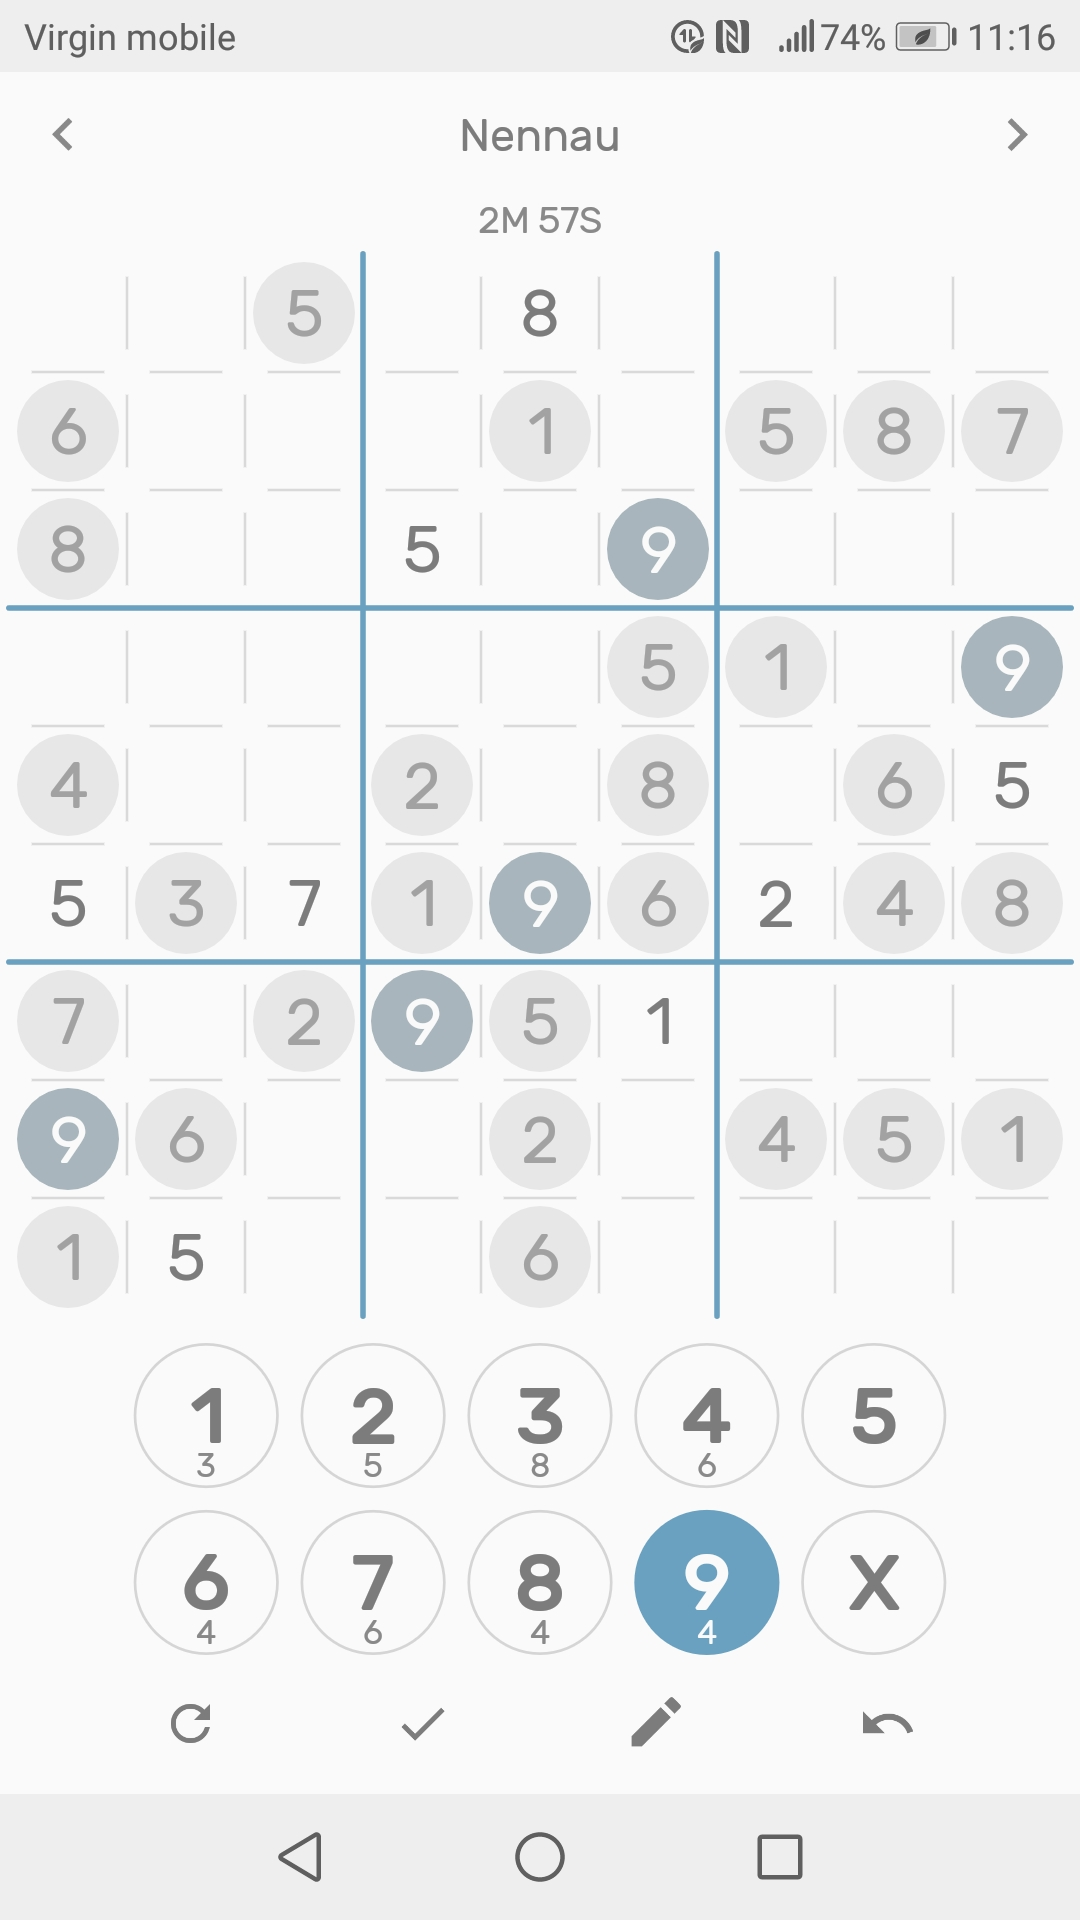
\includegraphics[width=\linewidth/2]{sudoku.jpg}
  \caption{Sudoku.}
  \label{fig:Sudoku1}
%\end{centering}
\end{figure}

Figure \ref{fig:Sudoku1} normal sudoku application.

\chapter{Requirements and tools}

\begin{itemize}
\item functional and nonfunctional requirements
\item use cases (UML diagrams)
\item description of tools
\item methodology of design and implementation
\end{itemize} 

\clearpage


\section{Functional requirements}
\par
There have been chosen to use both of previously mentioned approaches in the game, by creating a tutorial level with Sudoku 6 by 6 instead of 9 by 9. This way number of elements is decreased by over 55\%, so there are supposed to be two algorithms implemented: one for 6 on 6 and one for 9 on 9. Beside that the application will also need a validation to see if the Sudoku was solved correctly.
\par
Usage scenario:
%\par
\begin{enumerate}
	\item Instruction on how to play is played to the user(he can skip it if he wants to).
	\item User chose size of the Sudoku.
	\item User fills in the Sudoku.
	\item The program validates if the Sudoku is correct.
\end{enumerate}

\section{NonFunctional requirements}
\par
The user interface of the application should work similar to the way that Talkback is working: 
\begin{itemize}
\item Taping an element of Sudoku (number) should result in the interface reading the label to the user.
\item To edit an element, user must hold finger on it for a longer period of time, then the content of the element will be changed to the number that the element was tapped. 
\item In both cases, when the user try to edit a starting element (element that the game have started with), or when the user taps an empty element, a short message will be played to inform about it.
\end{itemize}
\par
To make it easier for blind user to find number on the screen of smartphone, and be aware of its localization,
\begin{itemize}
\item It should be possible to zoom in to one cell with only 6 or 9 elements (depending on the type of Sudoku).
\item It would be possible to move between cells by swipe events, and another after zooming out the swipe event can be used to go back to the menu.
\end{itemize}
\par
Other requirements:
\begin{itemize}
\item Turning on the TalkBack should not interfere with usage of the application.
\item Taking into account that this application can be used also by sand-blind people, there can be made a facilitation for them, by displaying white numbers on black background. With this contrast they will be easier to see.
\end{itemize}

\section {Description of tools\\{\large Tools used in works of the thesis}}%Methodology of design and implementation}

\par The chosen design tool is Android Studio with Java as the chosen programming language. Android Studio have been chosen as the most advanced tool in the field of creating android applications at that time. And Java was chosen due to the popularity of this programming language, which ensures wither range of existing solutions of many problems.

\chapter{External specification}
\begin{itemize}
\item hardware and software requirements
\item installation procedure
%\item activation procedure
\item types of users
\item user manual
%\item system administration
%\item security issues
\item example of usage
\item working scenarios (with screenshots or output files)
\end{itemize}

\clearpage
\section{Hardware and software requirements\\{Device required to use the application}}

\par The application requires a device with any version of  android.
Because the whole program uses only basic android functionalitis, there is no point in setting any higher version, this way the application will be available on more devices.


\section {Installation procedure\\{\large How to install}}

\par
The installation is based on downloading the APK file to the device and running the installation procedure appropriate to this device.

%\section {Activation procedure}

\section{Types of users}

\par This application has only one universal mode for all types of users. The Sudoku will still have simple visual elements, so the game could be played relying only on the eyesight. The content is read to the user that lets play the game without looking at the screen. And the white on black background contrast could help the partially blind players. This way the application is made as much accessible as it is possible.

\section{User manual\\{\large Application instruction}l}

\par 
All the basic instructions are shown and played every time after starting the application, and can be skipped with tapping the screen. 
\par
Editing the content of Sudoku number is enabled by a long tap, after long tapping the number it can be incremented by tapping it, after reaching the limit the number goes back to zero. Moving between cells to access more numbers is done by swipping a finger on the screen.
\par
When the talkback is on, the swipe must be done with two fingers.
\par 
At the beginning user is given a simple instruction on how to play the game:
\begin{quote}
Welcome to blind Sudoku!
Fill in the boxes so every number will be placed only
once in every row, column, and cell. Swipe your fingers to navigate between the cells,
and tap a box to hear its content. Long tap the box to enable editing the number, and tap
the box to increment the number. Double tap to continue. Have fun!
\end{quote}

%\section{System administration}

%\section {Security issues}

%\section {Example of usage}

\section {Working scenarios (with screenshots or output files)}

\par This application uses two xml views. One for the instructions and one for the cell filled with numbers.

\begin{figure}
\centering
  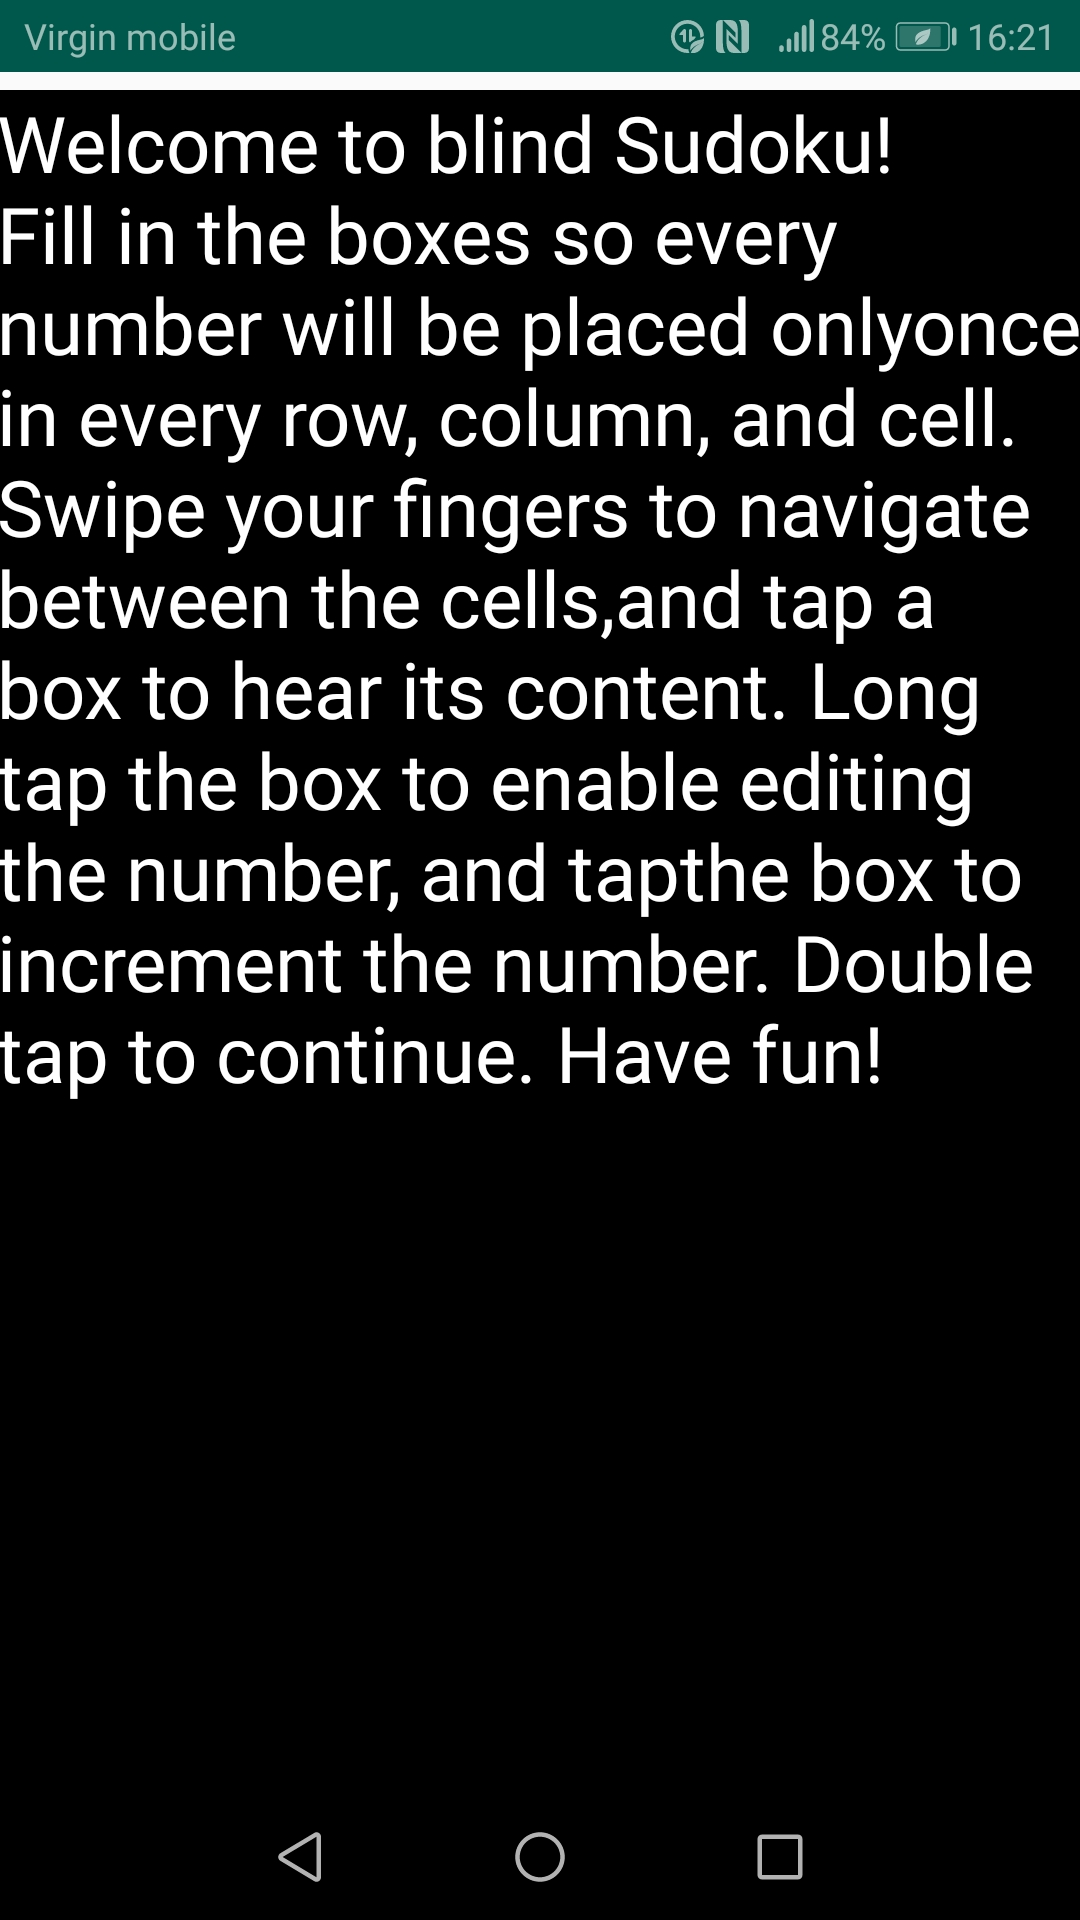
\includegraphics[width=\linewidth/2]{instructions.jpg}
  \caption{Instructions.}
  \label{fig:Game instructions}
%\end{centering}
\end{figure}

Figure \ref{fig:Game instructions} welcome message.

\begin{figure}
\centering
  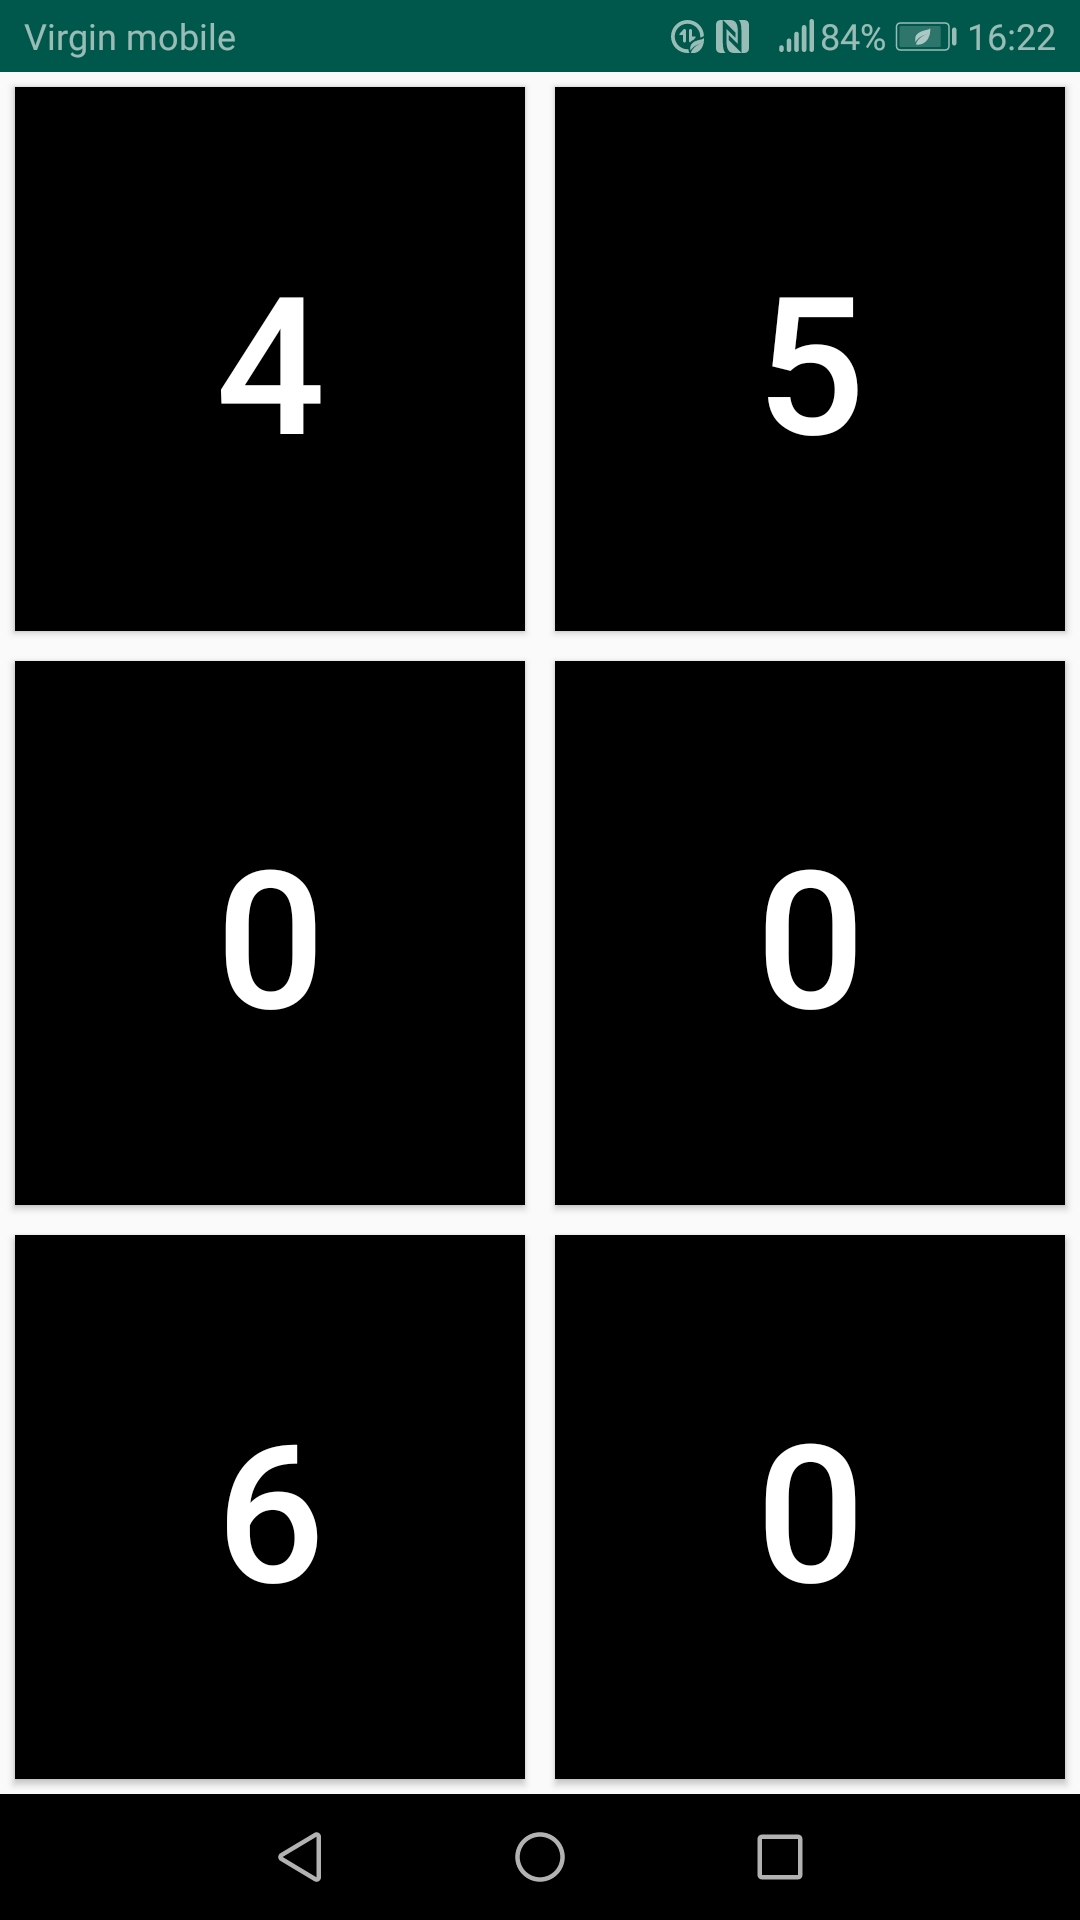
\includegraphics[width=\linewidth/2]{sudoku cell.jpg}
  \caption{Instructions.}
  \label{fig:Sudoku cell}
%\end{centering}
\end{figure}

Figure \ref{fig:Sudoku cell} game view with Sudoku cell.


\iffalse
\begin{comment}
\begin{figure}
\centering
\begin{tikzpicture}
\begin{axis}[
    y tick label style={
        /pgf/number format/.cd,
            fixed,   
            fixed zerofill, % 1.0 instead of 1
            precision=1,
        /tikz/.cd
    },
    x tick label style={
        /pgf/number format/.cd,
            fixed,
            fixed zerofill,
            precision=2,
        /tikz/.cd
    }
]
\addplot [domain=0.0:0.1] {rnd};
\end{axis} 
\end{tikzpicture}
\caption{A caption of a figure is \textbf{below} it.}
\label{fig:2}
\end{figure}
\end{comment}
\fi

\chapter{Internal specification}

\begin{itemize}
%\item concept of the system
%\item system architecture
%\item description of data structures (and data bases)
\item components, modules, libraries, resume of important classes (if used)
\item resume of important algorithms (if used)
\item details of implementation of selected parts
\item applied design patterns
\item UML diagrams
\end{itemize}


Use special environment for inline code, eg \lstinline|descriptor| or \lstinline|descriptor_gaussian|. 
Longer parts of code put in the figure environment, eg. code in Fig. \ref{fig:pseudokod}. Very long listings–move to an appendix.

\clearpage

%\section {Concept of the system}
%\section {System architecture}
%\section {Description of data structures }
\section {Components, modules, libraries, resume of important classes}

\par
The whole program is based mostly on two classes. The sudoku logic in class Sudoku made of: generating Sudoku, validating the Sudoku, and all the other methods needed to work with the Sudoku. The MainActivity class responsible for using the Sudoku class and connecting it to the other elements of the game.

\section {Resume of important algorithms}
\par
Generation of the 6 by 6 Sudoku was problematic, due to the fact that a square cannot be made of six square elements (what is required by most algorithms). This is why this program uses a simpler algorithm:
\begin{enumerate}
	\item Generate numbers from one to six in random order, and put them into the first row.
	\item Go to the next row.
	\item Copy the content of the previous row and: 
	\begin{enumerate}
   		 \item If the row number can be divided by 3, shift the numbers of this row by one place.
   		 \item If the row number can not be divided by 3, shift the numbers of this row by two places.
  	\end{enumerate}
	\item If the Sudoku is not full yet, go back to step number two.
	\item The Sudoku is ready.
\end{enumerate}

\par Later on the generated data is copied from one array to another during the copping process the correct indexes of the arrays are compared with a ready made SmallTemplate object to create holes for the user to fill in. Letter on both the first and the second array can be compared to see it the user solved the second correctly.

\par The application behavior with Talkback should be similar to the one with Talkback turned off as much as possible. Firstly the reading of buttons labels by Talkback was turned off, so it would be done by the implementation in the program. It was done by setting buttons android:importantForAccessibility to "no" in the XML file. Secondly the reaction to tapping the buttons had to be overeaten, so the user would not have to tap twice more times and to override the previously mentioned reading of labels. It was done by using the setOnHoverListener on buttons, and implementing there the same behavior as in the onClick method, where we test if the talkback is on by using the AccessibilityManager.

\section {Details of implementation of selected parts\\ {\large The most important parts of implementation}}

\par The game is based mostly on only one xml view, that is one Sudoku cell, with numbers changing after moving between cells, and editing the content inside them. After every swipe the current cell number is adjusted and the function updating the view, with data from Sudoku, is called.



%\section {Applied design patterns}
\section {UML diagrams}

\begin{figure}
\centering
  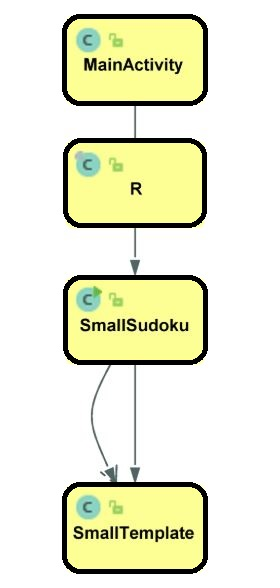
\includegraphics[width=\linewidth/2]{UML.jpg}
  \caption{UML diagram.}
  \label{fig:Diagram}
%\end{centering}
\end{figure}

Figure \ref{fig:Diagram} UML of the project.

\iffalse
\begin{comment}
\begin{figure}
\centering
\begin{lstlisting}
class descriptor_gaussian : virtual public descriptor
{
   protected:
      /** core of the gaussian fuzzy set */
      double _mean;
      /** fuzzyfication of the gaussian fuzzy set */
      double _stddev;
      
   public:
      /** @param mean core of the set
          @param stddev standard deviation */
      descriptor_gaussian (double mean, double stddev);
      descriptor_gaussian (const descriptor_gaussian & w);
      virtual ~descriptor_gaussian();
      virtual descriptor * clone () const;
      
      /** The method elaborates membership to the gaussian fuzzy set. */
      virtual double getMembership (double x) const;
     
};
\end{lstlisting}
\caption{The \lstinline|descriptor_gaussian| class.}
\label{fig:pseudokod}
\end{figure}
\end{comment}
\fi


\chapter{Verification and validation}
\begin{itemize}
\item testing paradigm (eg V model)
\item test cases, testing scope (full / partial)
\item detected and fixed bugs
\item results of experiments (optional)
\end{itemize}

 \clearpage

\section{Testing paradigm\\ {\large State of the testing metodology }}
 
\par Due to the importance of Talkback compatibility, every feature had to be tested with and without enabled Talkback.

\section{Test cases\\ {\large All the most important cases taken into account during testing }}

\begin{usecase}{User actions}
    \addrow{Edit empty box}{After long tapping the empty box the number editing is enabled, and every tap increments the number. After next long tap the content of box is saved.}

    \addrow{Edit box with content generated by application}{User is informed that the content cannot be changed.}

	\iffalse
    \addmulrow{Main path (M)}{
        \item User selects \ldots
        \item System demands \ldots}
	\fi
	\addrow{Single tap a box}{Application speaks the number that is inside the box.}
	\addrow{Single tap a box when Talkback is on}{Application speaks the number that is inside the box.}
	\addrow{Swipe vertically and horisontally}{The view moves between cells and stops and detects if it can move further.}
	\addrow{Fill in the Sudoku correctly}{Application informs that the Sudoku is correct.}
	\addrow{Fill in the Sudoku incorrectly}{Application informs that the Sudoku is incorrect.}
	
\end{usecase}

\section{Detected and fixed bugs\\ {\large All the bugs that have been detected during testing and development }}

\begin{enumerate}
	\item The upper limit for vertival cell movement was to high, that resulted in index out of bounds exception.
	\item The application was displaying wrong numbers due to a mistake in translation of button number into x and y coordinates of sudoku.
	\item Vertical swipe was not always working, because the event was not defined properly.
	\item Application was not able to compile. The first usage of the text to speech was accidentally before its initialization.
\end{enumerate}


\chapter{Conclusions}
\begin{itemize}
\item achieved results with regard to objectives of the thesis and requirements
\item path of further development (eg functional extension …)
\item encountered difficulties and problems
\end{itemize}

\clearpage

\section{Achieved results with regard to objectives of the thesis and requirements \\{\large Comparison between what was stated at the beginning as the goal and what was the final result}}

\par The final result of the project is fully functional Sudoku game that can be played without looking at the screen. It can work both with and without turned on Talkback, and the accessibility feature would not change. The only difference in playing the game with Talkback turned on is the way player enables the change of number in button. Instead of just holding the button for a longer period of time, it must be double tapped where the second tap is the one to be held longer.

\section{Path of further development \\{\large Suggestions for what can be done more with the game}}

\par At this time the game can be played only on small (six on six) Sudoku with simple algorithm of generation, for better game play results it could be possible to chose size of Sudoku and level of difficulty. The application could be also extended by additional features not necessary for the game mechanics like saving time of the play into a ranking to compere results. Possibility to see the ranking should be made in the menu view, that would be also useful to implement together with going back to menu from the game view.
\par There are also other features that could make the game more accessible. Possibility of showing the whole Sudoku on the screen, by making the zoom out gesture, and zoom in to go back into the single cell. When the whole Sudoku is visible it is easier to look thru rows and columns, but navigating between 36 elements (or even 81 if the nine on nine version was chosen) could be challenging for a blind person, so both zoom in and zoom out views should be available. Similar result can be achieved by implementing hints for the user: Telling him if there is a certain number in a row or column. How many occurrences of a certain numbers missing in the whole Sudoku. It could also read all numbers in a row or column in the same order as they are placed in the Sudoku.
\par Leaving the subject of the game itself, there is also place for improvement in the displaying the text. The contrast of white text on black background can help people who still have partial sight, but for large variety of eyesight diseases, it can be possible that for some eyesight disease it would be easier to read with different contrast. This is why it should be possible to change the colors of contrast in the menu settings.

\section{Encountered difficulties and problems}

\par The most difficult part of implementing this application was making the application behavior, with and without Talkback, as similar as possible. There were many aspects that had to be taken into account, as many normal behaviors of the phone are overwritten when the Talkback is on.


 \iffalse
\begin{table}
\centering
\caption{A caption of a table is \textbf{above} it.}
\label{id:tab:wyniki}
\begin{tabular}{rrrrrrrr}
\toprule
	         &                                     \multicolumn{7}{c}{method}                                      \\
	         \cmidrule{2-8}
	         &         &         &        \multicolumn{3}{c}{alg. 3}        & \multicolumn{2}{c}{alg. 4, $\gamma = 2$} \\
	         \cmidrule(r){4-6}\cmidrule(r){7-8}
	$\zeta$ &     alg. 1 &   alg. 2 & $\alpha= 1.5$ & $\alpha= 2$ & $\alpha= 3$ &   $\beta = 0.1$  &   $\beta = -0.1$ \\
\midrule
	       0 &  8.3250 & 1.45305 &       7.5791 &    14.8517 &    20.0028 & 1.16396 &                       1.1365 \\
	       5 &  0.6111 & 2.27126 &       6.9952 &    13.8560 &    18.6064 & 1.18659 &                       1.1630 \\
	      10 & 11.6126 & 2.69218 &       6.2520 &    12.5202 &    16.8278 & 1.23180 &                       1.2045 \\
	      15 &  0.5665 & 2.95046 &       5.7753 &    11.4588 &    15.4837 & 1.25131 &                       1.2614 \\
	      20 & 15.8728 & 3.07225 &       5.3071 &    10.3935 &    13.8738 & 1.25307 &                       1.2217 \\
	      25 &  0.9791 & 3.19034 &       5.4575 &     9.9533 &    13.0721 & 1.27104 &                       1.2640 \\
	      30 &  2.0228 & 3.27474 &       5.7461 &     9.7164 &    12.2637 & 1.33404 &                       1.3209 \\
	      35 & 13.4210 & 3.36086 &       6.6735 &    10.0442 &    12.0270 & 1.35385 &                       1.3059 \\
	      40 & 13.2226 & 3.36420 &       7.7248 &    10.4495 &    12.0379 & 1.34919 &                       1.2768 \\
	      45 & 12.8445 & 3.47436 &       8.5539 &    10.8552 &    12.2773 & 1.42303 &                       1.4362 \\
	      50 & 12.9245 & 3.58228 &       9.2702 &    11.2183 &    12.3990 & 1.40922 &                       1.3724 \\
\bottomrule
\end{tabular}
\end{table}  
\fi
 

 


%%%%%%%%%%%%%%%%%%%%%%%%%%%%%%%%%%%%%%%%%%
\backmatter
\pagenumbering{Roman}
\stepcounter{PagesWithoutNumbers}
\setcounter{page}{\value{PagesWithoutNumbers}}

\pagestyle{onlyPageNumbers}

%%%%%%%%%%% bibliography %%%%%%%%%%%%
\bibliographystyle{plain}
\bibliography{bibliography}

%%%%%%%%%  appendices %%%%%%%%%%%%%%%%%%% 

\begin{appendices} 


 

\chapter*{List of abbreviations and symbols}

\begin{itemize}
\item[DNA] deoxyribonucleic acid
\item[MVC] model--view--controller 
\item[$N$] cardinality of data set
\item[$\mu$] membership function of a fuzzy set
\item[$\mathbb{E}$] set of edges of a graph
\item[$\mathcal{L}$] Laplace transformation
\end{itemize}


\chapter*{Listings}

(Put long listings in the appendix.)

\begin{lstlisting}
partition fcm_possibilistic::doPartition
                             (const dataset & ds)
{
   try
   {
      if (_nClusters < 1)
         throw std::string ("unknown number of clusters");
      if (_nIterations < 1 and _epsilon < 0)
         throw std::string ("You should set a maximal number of iteration or minimal difference -- epsilon.");
      if (_nIterations > 0 and _epsilon > 0)
         throw std::string ("Both number of iterations and minimal epsilon set -- you should set either number of iterations or minimal epsilon.");
   
      auto mX = ds.getMatrix();
      std::size_t nAttr = ds.getNumberOfAttributes();
      std::size_t nX    = ds.getNumberOfData();
      std::vector<std::vector<double>> mV;
      mU = std::vector<std::vector<double>> (_nClusters);
      for (auto & u : mU)
         u = std::vector<double> (nX);
      randomise(mU);
      normaliseByColumns(mU);
      calculateEtas(_nClusters, nX, ds);
      if (_nIterations > 0)
      {
         for (int iter = 0; iter < _nIterations; iter++)
         {
            mV = calculateClusterCentres(mU, mX);
            mU = modifyPartitionMatrix (mV, mX);
         }
      }
      else if (_epsilon > 0)
      {
         double frob;
         do 
         {
            mV = calculateClusterCentres(mU, mX);
            auto mUnew = modifyPartitionMatrix (mV, mX);
            
            frob = Frobenius_norm_of_difference (mU, mUnew);
            mU = mUnew;
         } while (frob > _epsilon);
      }
      mV = calculateClusterCentres(mU, mX);
      std::vector<std::vector<double>> mS = calculateClusterFuzzification(mU, mV, mX);
      
      partition part;
      for (int c = 0; c < _nClusters; c++)
      {
         cluster cl; 
         for (std::size_t a = 0; a < nAttr; a++)
         {
            descriptor_gaussian d (mV[c][a], mS[c][a]);
            cl.addDescriptor(d);
         }
         part.addCluster(cl);
      }
      return part;
   }
   catch (my_exception & ex)                                  
   {                                                       
      throw my_exception (__FILE__, __FUNCTION__, __LINE__, ex.what()); 
   }                                                          
   catch (std::exception & ex)                                 
   {                                                            
      throw my_exceptionn (__FILE__, __FUNCTION__, __LINE__, ex.what()); 
   }                                                            
   catch (std::string & ex)                                     
   {                                                            
      throw my_exception (__FILE__, __FUNCTION__, __LINE__, ex);        
   }                                                             
   catch (...)                                                   
   {                                                             
      throw my_exception (__FILE__, __FUNCTION__, __LINE__, "unknown expection");       
   }  
}
\end{lstlisting} 

\chapter*{Contents of attached CD}

The thesis is accompanied by a CD containing:
\begin{itemize}
\item thesis (\LaTeX\ source files and final \texttt{pdf} file),
\item source code of the application,
\item test data.
\end{itemize}
 

\listoffigures
\listoftables
	
\end{appendices}


\end{document}


%% Finis coronat opus.